\chapter{\uppercase{Background on Data-Consistent Inversion} \label{chapter:02}}

\section{Notation, Terminology, and Assumptions}

We begin by assuming that a (deterministic) model, denoted by $$\M (u, \param) = 0,$$ is specified to relate observable state variables $u$ to model inputs ({\em parameters}) denoted by the vector $\param\in\RP$.
The components $\param_\iparam$ may include parameters in either the model operator (e.g. a diffusion coefficient) or input data (e.g. the frequency of a sinusoidal source, initial, or boundary information).
We allow $\pspace$ to denote the set of all possible input parameters. 
We assume $\pspace\subset\RP$ is equipped a (volume) measure, $\pmeas$ on the Borel $\sa$ $\pborel$, defining the measure space $\Pspace$.
The solution operator of the model $\M$ then defines a map taking $\param\in\pspace$ to a solution denoted $u\lam$ which is assumed to be unique. 

However, in real experimental settings we are often unable to observe $u\lam$, instead having access to some finite set of observable scalar quantities. 
For example, in experiments involving the diffusion of heat, we can typically only record the temperature at some small number of pre-specified points in space-time where measurement devices can be positioned.

Such observable values of $u\lam$ are mathematically modeled by functionals of the solution, denoted $\qoi_\idata: u\lam \to \RR$.
The collection of such functionals into a vector defines a {\em Quantity of Interest} (QoI) map. 
Since the solution to the model depends on $\param$, so do the QoI, which motivates the notation 
$$\qlam := \qoi( u\lam ) \in\RD,$$
to make this dependence on model parameters explicit.
Furthermore, this convention captures a realistic limitation of an experimental setting, where we may be able to control $\param$ in order to observe $\qlam$, but lack the ability to observe $u\lam$ directly.
The outputs of the QoI map $\qlam = \data$ are what we refer to as the \emph{data}. 
Similarly, the range of the QoI defines the \emph{data space} $\dspace$, i.e. 
$$\dspace = \qoi(\pspace) \subset \RD$$

We let $\qspace$ denote the set of possible QoI maps for which it is possible to collect experimental data.
For example, suppose we may record only a single temperature measurement at any of ten locations in space-time.
Then $\qspace$ is defined by ten possible QoI maps. 
If we can record any two such measurements, then $\qspace$ is defined by $\binom{10}{2} = 45$ possible maps.
Observe that $\qspace$ could easily be uncountable, for example if we were not limited to the spatial locations (or time) at which we could record temperature measurements.
However, for simplicity, we will only discuss problems where $\qspace$ is finite.
In the event that we need to compare maps, we adopt the notation $\dspace_{\qoi}$ to emphasize that the data space depends on the choice of QoI map $\qoi$; when the context is clear, we drop the subscript.
The only assumption on $\qoi$ that we impose throughout this work is that of piecewise-differentiability.


%%%%%%%%%%%%%%%%%%%%%%%%%%%%%%%%%%%%%%%%%%%%%%%%%%%%%%%%%%%%%%%%%%%%%%


\
\section{Set-Based Inversion for Measures}\label{sec:ch02-set}

To properly summarize the Stochastic Inverse Problem (SIP) and desired solution, we define several measure/probability spaces and refer to the schematic given in Figure \ref{fig:scheme}\---borrowed from \cite{BM17}\---in order to illustrate the steps and spaces required in the formulation and solution of the SIPs we consider herein.
For a more extensive review, we refer the reader to \cite{BBE11}, \cite{BES12}, \cite{BET+14}, and \cite{BM17}. 

%%%%%%%%%%%%%%%%%%%%%%%%
\begin{figure}[!h]
\begin{equation}
\underbrace{
\underbrace{
\overbrace{ 
 \Pspace \xmapsto{\  Q \ } \Dspace
  \xmapsto{\ \dataP \ } (\dspace, \dborel, \dataP)
 }^{
 \text{(S1): Stochastic Inverse Problem (SIP)}
 }
 \xmapsto{\ Q^{-1} \ } (\pspace, \cborel, \contourP)
 }_{
 \text{(S2): Solution to SIP Satisfying Eq. \eqref{eq:dataspace_pushforward_measure}}} 
 \xmapsto{\ \set{\PP_\ell}_{\ell\in\mathcal{L}} \ } (\pspace, \pborel, \paramP)
 }
 _{
 \text{(S3): Unique Solution to SIP by Eq.~\eqref{eq:disintegration_measure} and Ansatz}
 }
\end{equation}
\caption{The first step (S1) defines (i)~the formulation of the SIP by specification of the model, (ii)~the measure spaces of parameters and (iii)~observable outputs, and (iv)~the probability measure on the latter. The second step (S2) defines a unique solution to the SIP on the space $\pspace$ equipped with the contour $\sa$ $\cborel$ using the definition of the push-forward measure. In (S3), the Disintegration Theorem and and Ansatz are applied to define a unique solution on the space of interest $(\pspace, \pborel)$ equipped with a probability measure $\paramP$.}
\label{fig:scheme}
\end{figure}


The initial measure/probability spaces involved in the formulation of the SIP are summarized in step (S1) of Fig.~\ref{fig:scheme}, starting with measure space $\Pspace$.

The assumption that $\qoi$ is at least piecewise-differentiable implies the measurability of the QoI map, so that the space $\dspace$ induced by $\qoi$ is equipped with the Borel $\sa$ $\dborel$ [TK - cite textbook].
The ``push-forward'' measure $\dmeas$ on ${(\dspace, \dborel)}$ is defined as 
\begin{equation}\label{eq:dataspace_pushforward_measure}
\dmeas (A) = \int_A \, d\dmeas := \int_{\qoi^{-1}(A)} \, d\pmeas = \pmeas \left (\qoi^{-1}(A) \right ) \quad \forall \;  A\in\dborel,
\end{equation}
which defines the measure space $\Dspace$\footnote{When referring to properties of the data space that are not unique to the choice of map used to induce $\dspace$, we will drop the subscript notation and assume the dependence is understood, as expressed in Fig.~\ref{fig:scheme}.}.
The push-forward distribution $\partial \dataP / \partial \mu_D$ is referred to as the \emph{predicted} distribution and is given by the Radon-Nikodym derivative with respect to (the Lebesgue) volume measure $\mu_D$ on ${(\dspace, \dborel)}$ 

The final step in (S1) involves the specification of a probability measure $\dataP$ on ${(\dspace, \dborel)}$ to model the uncertainty in data. 
We colloquially refer to the distribution (given by the Radon-Nikodym derivative $\partial \dataP / \partial \pmeas$) as the \emph{observed} distribution, where $\pmeas$ is taken to be the (Lebesgue) volume measure on ${(\pspace, \pborel)}$. 
This leads to the following SIP: determine a probability measure $\paramP$ on ${(\pspace, \pborel)}$ such that the push-forward measure of $\paramP$ matches $\dataP$. 

In other words, determine a $\paramP$ satisfying
\begin{equation}\label{eq:inverse_measure}
\paramP \left ( \qoi^{-1}(E)\right ) = \PP_{\dspace}(E) \; \forall \, E \in \dborel.
\end{equation}

We call any such solution $\paramP$ to Eq.~\eqref{eq:inverse_measure} a (measure-theoretic) solution to the SIP.
This equation implies that any solution is uniquely determined on the induced contour $\sa$ 
\begin{equation}\label{eq:contour_sa}
\cborel = \set{\qoi^{-1}(E) : E \in \dborel } \subset \pborel,
\end{equation}
which is summarized as step (S2) of Fig.~\ref{fig:scheme}. 

However, for sets $A \in \pborel \setminus \cborel$, more information is required than is provided in Eq.~\eqref{eq:inverse_measure} in order to determine $\paramP (A)$. 
By the Implicit Function Theorem, if $\data \in C^1 (\pspace)$ and we let $\data\in\dspace$ be a fixed datum, $\qoi^{-1}(q)$ exists as a $(\nparams-\ndata)$\--dimensional manifold (possibly piecewise-defined) that we refer to as a \emph{generalized contour} \cite{BET+14}. 
These generalized contours can be indexed by a manifold (also possibly piecewise-defined) of dimension $\ndata$ called a \emph{transverse parameterization} that intersects each contour once and only once. 
In \cite{BET+14}, it is shown that transverse parameterizations are guaranteed to exist but are in general not unique.

We let $\LL$ denote any particular transverse parameterization. 
Each $\ell\in\LL$ corresponds to a unique generalized contour $\CC_\ell \in \pspace$ and each point $\param\in\pspace$ belongs to a unique $\CC_\ell\in\pspace$.
Thus, a transverse parameterization defines a bijection between the manifold $\LL$ and the partitioning of $\pspace$ into generalized contours. 
The induced $\sa$ $\cborel$ and this bijection can then be used to define the measurable space $(\LL, \BB_\LL)$. 

We denote the projection map $P_\LL :\pspace \to \LL$, and let $\set{\CC_\ell}_{\ell\in\LL}$ represent the family of generalized contours indexed by $\LL$, yielding the associated family of measurable spaces $\set{\left ( \CC_\ell, \BB_{\CC_\ell} \right )}_{\ell\in\LL}{}$. 
A Disintegration Theorem [TK - cite] is then leveraged to define a unique decomposition for any $\paramP$ defined on $(\pspace, \pborel)$ as a (marginal) probability measure $\PP_\LL$ on $(\LL, \BB_\LL)$ and a family of (conditional) probability measures $\set{\PP_\ell}_{\ell\in\LL}$ on $\set{\left ( \CC_\ell, \BB_{\CC_\ell} \right )}_{\ell\in\LL}$ such that 
\begin{equation}\label{eq:disintegration_measure}
\paramP (A) = \int_{P_\LL(A)} \left ( \int_{P_{\LL}^{-1} (\ell) \cap A}\, d\PP_\ell(\param) \right )\, d\PP_\LL (\ell), \; \forall \; A \in \pborel 
\end{equation}


The uniqueness of a probability measure $\paramP$ on ${(\pspace, \cborel)}$ satisfying Eq.~\eqref{eq:inverse_measure} implies the uniqueness of the marginal probability measures $\PP_\LL$ for any particular specification of $\dataP$ on ${(\dspace, \dborel)}$. 
The disintegration of Eq.~\eqref{eq:disintegration_measure} implies that a specification of a family of conditional probability measures $\set{P_\ell}_{\ell\in\LL}$ gives us a unique solution to the SIP on ${(\CC_\ell, \BB_{\CC_\ell})}$.
 
However, the conditional measures cannot be determined by solely by the specification of $\data\in\dspace$. 
We follow the work of \cite{BET+14} and adopt the \emph{standard ansatz} determined by the disintegration of the volume measure $\pmeas$ to compute probabilities of sets contained within contour events. 
The standard ansatz is given by 
\begin{equation}\label{eq:standard_ansatz}
\PP_\ell = \mu_{\CC_\ell} / \mu_{\CC_\ell}(\CC_\ell), \; \forall \; \ell \in \LL,
\end{equation}
where $\mu_{\CC_\ell}$ is the disintegrated volume measure on generalized contour $\CC_\ell$.
Thus, we have defined a unique solution to the SIP on ${(\pspace, \pborel)}$, completing step (S3) in Fig.~\ref{fig:scheme}. 


%%%%%%%%%%%%%%%%%%%%%%%%%%%%%%%%%%%%%%%%%%%%%


\subsection{Numerical Approximation and Analysis}\label{sec:set-approx}
In the \emph{set-based} inversion framework, there are two primary sources of approximation error: 
\begin{description}[leftmargin=!, labelwidth=0.7in]
  \item[(1)] partitioning the parameter space $\pspace$ to approximate events in $\cborel$ and $\pborel$, and
  \item[(2)]  partitioning the data space $\dspace$ to approximate events in $\dborel$.
\end{description}
In practice, we must rely on a finite numerical approximation of the (often uncountable) events in the $\sa$s $\dborel$, $\cborel$, and $\pborel$.
Owing to the inclusion $\cborel \subset \pborel$, it is possible to approximate events in both of these $\sa$s simultaneously. 

Assume we fix some collection of sets $\set{D_\idisc}_{\idisc=1}^{\ndiscs} \subset \dborel$ to partition $\dspace$ (independent of any specification of $\qoi$), and that we partition $\pspace$ with $\set{\VV_\iparam}_{\iparam=1}^{\nsamps}$, where $\VV_\iparam \in \pborel$. 
Both sets yield implicitly-defined Voronoi-cell partitions given by a finite sampling of each space.
In order to approximate $\paramP(\VV_\iparam)$ for $\iparam=1,\hdots,\nsamps$, we must determine which collection of $\VV_\iparam$'s approximate $\qoi^{-1}(D_\idisc)$ for each $\idisc=1,\hdots,\ndiscs$, and then apply the ansatz on this approximation of the contour event with known probability $\dataP(D_\idisc)$.
Algorithm~\ref{alg:inv_density} was proven to converge to the solution $\paramP$ in \cite{BET+14-arxiv} as the discretizations of $\pspace$ and $\dspace$ (as ${\nsamps \text{ and } \ndiscs}$ tend to $\infty$, respectively. 


\subsubsection{Algorithm}\label{sec:set-algorithm}
We present a non-intrusive algorithm based on Monte-Carlo sampling\---initially introduced in \cite{BET+14} and further analyzed in \cite{BET+14-arxiv}\---that is structured in four stages (written as four independent for-loops) that are linked to the stages in Fig.~\ref{fig:scheme}. 
We direct the interested reader to \cite{BET+14-arxiv} for more detailed information and analysis of this algorithm, e.g., on the requirement of a sampler being ``$\pborel$-consistent'' to ensure convergence. 


\begin{algorithm}[hbtp]
\DontPrintSemicolon
Choose a discretization partition $\set{D_\idisc}_{\idisc=1}^{\ndiscs}$ of $\dspace$.\\
	\For{$\idisc = 1, \hdots, \ndiscs$}{
			Compute $p_{\dspace, \idisc} = \dataP(D_\idisc)$.
	}
	Choose samples $\set{\param^{(\iparam)}}_{\iparam=1}^{\nsamps} \subset \pspace$, which implicitly defines a Voronoi-cell partition $\set{\VV_\iparam}_{\iparam=1}^{\nsamps}$ of $\pspace$.\\
	\For{$\iparam = 1, \hdots, \nsamps$}{
	Compute quantity of interest vectors $\qoi_\iparam = \qoi(\param^{(\iparam)})$.\\
	Bin $\qoi_\iparam$ in the partition $\set{D_\idisc}_{\idisc=1}^{\ndiscs}$ and let $\OO_\iparam = \set{i: \qoi_\iparam \in D_\idisc}$.\\
	Compute approximations $V_\iparam \approx \pmeas (\VV_\iparam)$.
	}
	\For{$\idisc = 1, \hdots, \ndiscs$}{
	Compute $\CC_\idisc = \set{\iparam:Q_\iparam \in D_\idisc}$.
	}
	\For{$\iparam = 1, \hdots, \nsamps$}{
	Compute $p_{\pspace, \iparam} = \left ( V_\iparam / \sum_{j\in \CC_{\OO_\iparam} } V_j \right ) p_{\dspace, \OO_\iparam}$.
	}
	For any $A\in \pborel$, compute 
	\begin{equation}
	\PP_{\pspace, \ndiscs, \nsamps} (A) = \sum_{\iparam=1}^\nsamps p_{\pspace, \iparam} \Chi_{\VV_\iparam} (A) 
	\end{equation}
 \caption{Numerical Approximation of the Inverse Density}
 \label{alg:inv_density}
\end{algorithm}
\FloatBarrier

The first two stages correspond to formulating the discretized version of the SIP given in step (S1) in Fig.~\ref{fig:scheme}. 
We first discretize the probability space $(\dspace, \dborel, \dataP)$.
Then, we simultaneously discretize the measure space $(\pspace, \pborel, \pmeas)$ and construct a simple-function approximation to the map $\qoi$.
These stages introduce the primary sources of error, and the third and fourth stages may be thought of as solving the discretized SIP exactly.

The third stage then identifies the collection of Voronoi cells in $\pspace$ that approximate the contour events defined by $\qoi^{-1}(D_\idisc)$ for $\idisc=1,\hdots,\ndiscs$. This allows us to formulate the consistent solution to the SIP on $(\pspace, \cborel, \paramP)$ as illustrated in step (S2) of Fig.~\ref{fig:scheme}. 
Finally, the fourth stage constructs a discretized approximation to step (S3) in Fig.~\ref{fig:scheme} and uses a discrete version of the ansatz to approximate the probability of $\VV_\iparam$ for $\iparam=1,\dots,\nsamps$. 
This results in an approximate probability measure $P_{\pspace, \ndiscs, \nsamps}$ which produces the same probability estimates for events $A$ and $A\setminus \set{ \pspace^{(\iparam)} }_{\iparam=1}^\nsamps$, which are identical almost everywhere with respect to $\pmeas$. 

Note that Algorithm~\ref{alg:inv_density} is independent of the methods by which the samples $\set{ \pspace^{(\iparam)} }_{\iparam=1}^{\nsamps}$ were generated or sets in $\set{D_\idisc}_{\idisc=1}^{\ndiscs}$ are chosen.  
A thorough discussion of the choices involved in making such decisions is beyond the scope of this work, though we touch briefly on the discretization of $\dspace$ below. 



\subsection{Descriptions of Error}\label{sec:set-error}
Recall that we assumed $\dataP$ is absolutely continuous with respect to $\dmeas$, which allows us to describe $\dataP$ with a density $\rho_\dspace$. Then, for any partition $\set{D_\idisc}_{\idisc=1}^{\ndiscs}$ of $\dspace$, 
\[
\dataP (D_\idisc) = \int_{D_\idisc} \rho_\dspace \, \dmeas, \quad \text{ for } \idisc = 1, \hdots, \ndiscs.
\]

We often use Monte Carlo approximations to compute the approximations $p_{\dspace, \idisc}=\dataP(D_\idisc)$ in the first for-loop in Algorithm~\ref{alg:inv_density}. 
These samples are generated on $\dspace$ and do not require numerical solutions to the model. 
We therefore assume that for any discretization of $\dspace$, these approximations can be made sufficiently accurate and neglect the error in this computation. 

We denote the exact solution to the SIP associated with this partitioning of $\dspace$ by $\PP_{\pspace, \ndiscs}$. 
Approximate solutions to the SIP given in the final for-loop of Algorithm~\ref{alg:inv_density} are denoted by $\PP_{\pspace, \ndiscs, \nsamps, h}$.
Here, the $h$ is in reference to a mesh or other numerical parameter that determines the accuracy of the numerical solution $u_h(\param^{(\iparam)})\approx u(\param^{(\iparam)})$, and subsequently the accuracy in the computations of $\qoi_\iparam = \qoi(\param^{(\iparam)})$ in Algorithm~\ref{alg:inv_density}.
 
We assume that $h$ is tunable so that
\[
\lim\limits_{h \downarrow 0} \PP_{\pspace, \ndiscs, \nsamps, h} = \PP_{\pspace, \ndiscs, \nsamps}.
\]
In \cite{BM17}, the focus was on proving the convergence of $\PP_{\pspace, \ndiscs, \nsamps, h} (A) \to \paramP (A)$ for some $A\in \pborel$ and on estimating the error in $P_{\pspace, \ndiscs, \nsamps, h}(A)$.
There, as well as in \cite{BGE+15}, adjoint-based a posteriori estimates in the computed QoI are combined with a statistical analysis to both estimate and bound the error in $\PP_{\pspace, \ndiscs, \nsamps, h} (A)$.
In \cite{BM17}, adjoints were used to compute both error and derivative estimates of $\qoi(\param^{(\iparam)})$ to improve the accuracy in $\PP_{\pspace, \ndiscs, \nsamps, h} (A)$.
However, no work has to date fully explored the \emph{convergence rates} of Algorithm \ref{alg:inv_density}.
Furthermore, no work has yet to establish that these rates are independent of the choice of QoI map despite other studies establishing that the absolute error is very much affected by the geometric properties of the QoI maps \cite{BE13}.

In order to study convergence, we need to define a notion of distance on the space of probability measures on $\pspace$, which we denote by $\PPspace$. 
% There are many choices available to us and we discuss several useful metrics on $\paramP$ in Section~\ref{sec:metrics}. 
We will be using the Total Variation metric throughout this work, but for the time being, let $d$ represent a metric on $\PPspace$.

Then, we have by repeated application of the triangle inequality that
\begin{equation}
\label{eq:set-triangleineq}
d(\PP_{\pspace, \ndiscs, \nsamps, h}, \paramP) \leq 
\underset{ \text{(E1)} }{\underbrace{d(\PP_{\pspace, \ndiscs, \nsamps, h},\PP_{\pspace, \ndiscs, \nsamps})}} + 
\underset{ \text{(E2)} }{\underbrace{d(\PP_{\pspace, \ndiscs, \nsamps}, \PP_{\pspace, \ndiscs}) }}+ 
\underset{ \text{(E3)} }{\underbrace{d(\PP_{\pspace, \ndiscs}, \paramP) }}.
\end{equation}

The term (E1) describes the effect of the error in the numerically evaluated $\qoi_\iparam$ on the solution to the SIP. 
The term (E2) describes the effect of finite sampling error in $\pspace$ on the solution to the SIP and (E3) describes the effect of discretization error of $\dataP$ on the solution to the SIP. 

\subsection{Example}\label{sec:set-example}

2D identity map, known observed (square in center with area 1/100, i.e. density value of 100).

\vspace{3in}

%%%%%%%%%%%%%%%%%%%%%%%%%%%%%%%%%%%%%%%%%%%%%%%%%%%%%%%%%%%%%%%%%%%%%%



\
\section{Sample-Based Inversion for Measures}\label{sec:ch02-sample}
[TK - Words]

\begin{equation}
\updatedP = \initialP \frac{\observedP}{\predictedP}
\end{equation}

\begin{equation}
\begin{split}
\dci\\
\dciP\\
\dciD
\end{split}
\end{equation}

In place of the ansatz, we have an initial distribution.

\subsection{Numerical Approximation and Analysis}\label{sec:sample-approx}


\vspace{2in}

\subsection{Descriptions of Error}\label{sec:sample-error}

KDE is now the primary source, show relevant triangle inequality here.
Summarize Troy and Tim's work on the sensitivity analysis of everything.


Then, we have by repeated application of the triangle inequality that
\begin{equation}
\label{eq:sample-triangleineq}
d(\PP_{\pspace, \ndiscs, \nsamps, h}, \paramP) \leq 
\underset{ \text{(E1)} }{\underbrace{d(\PP_{\pspace, \ndiscs, \nsamps, h},\PP_{\pspace, \ndiscs, \nsamps})}} + 
\underset{ \text{(E2)} }{\underbrace{d(\PP_{\pspace, \ndiscs, \nsamps}, \PP_{\pspace, \ndiscs}) }}+ 
\underset{ \text{(E3)} }{\underbrace{d(\PP_{\pspace, \ndiscs}, \paramP) }}.
\end{equation}

Talk more about it.

\vspace{2in}

\subsection{Example}\label{sec:sample-example}
Identity Map in two dimensions
\vspace{3in}

%%%%%%%%%%%%%%%%%%%%%%%%%%%%%%%%%%%%%%%%%%%%%%%%%%%%%%%%%%%%%%%%%%%%%%

\
\section{Software Contributions}\label{sec:ch02-software}

\subsection{Background and Motivation}
The open-source software package BET was developed actively from 2012-2015 as part of research performed under grant [TK grant-DOE].
It was originally written in Python 2.7 and is administered by the Computational Hydrology Group at the University of Texas: Austin through their UT-CHG GitHub group [TK - cite Github]. 
The purpose of this open-source software package was to implement the methods first described in [TK - cite BET papers] for the description and solution of stochastic inverse problems. 

In the intermittent years since its original publication in [TK - date of first release, cite Github], the BET package has seen two major releases and the incorporation of several sub-modules (e.g. the functions in {\tt sensitivity} implement much of the original research performed by Dr. Walsh [TK - cite Scott]). 
Since the last major release [TK - cite latest release], the Python community announced the end of long-term support for Python 2 [TK - cite announcement]. 
Several of the dependencies in BET have been actively developed in Python 3 with no updates to the Python 2 analogs, which suggested that BET should likely undergo the same transition.

The work summarized in Section~\ref{sec:ch02-sample} was implemented in Python 3 independently by the author through the release of the ConsistentBayes package.
Since that code was used for many of the results that constituted the preliminary results for this work, it made very litle sense to re-implement them in Python 2 for BET given the recent trends in community development. 
With funding made available through NSF [TK - cite grant], the opportunity to upgrade BET to Python 3 was the most sensible choice. 

The upgrade to Python 3.4+ began in January 2019 as a first step to incorporate the new sample-based method into BET. 
It was completed in late February. 
Major release 2.1.0 [TK - put in release] was designed to provide backwards-compatibility with the Python 2.7 version. 
Future installation specifications would not limit the versions of some core dependencies in order to provide backwards-compatibility with Python 2 (e.g. {\tt numpy}, {\tt scipy}) since this would likely downgrade previously installed software for end-users. 

Basic plotting functionality is demonstrated in iPython notebooks, which have seen an exponential growth rate on GitHub, and can be edited by the end-user to work with different plotting library versions and backends.




\
\section{Illustrative Examples}\label{sec:ch02-examples}
In our examples, we do not work with any model and make observations $\qoi$ directly on the parameter space $\pspace$, so term (E1) in Eq.~\eqref{eq:set-triangleineq} is identically zero for the examples we present in Section \ref{sec:results}.
Furthermore, since the probabilities we introduce on $\dspace$ in the numerical results are uniform and our maps linear, the densities can be described analytically with a characteristic function and so the solution to the SIP $\paramP$ can be given exactly by a change of variables formula, which we present later. 
Generally, what we assume is that $\ndiscs$ is chosen without respect to $\nsamps$ so that (E3) = $d(P_{\pspace, \ndiscs}, P_\pspace)$ has been made sufficiently small. 
This effectively amounts to saying that the decision about how to discretize the uncertainty in $\dspace$ is made a priori to cater top some problem specifications. 

Therefore, we focus our attention on the source of error introduced by $d(P_{\pspace, \ndiscs, \nsamps}, P_{\pspace, \ndiscs} )$, the primary contribution of error in Eq.~\eqref{eq:set-triangleineq}, which is given by the term $d(P_{\pspace, \ndiscs, \nsamps}, P_{\pspace, \ndiscs})$.
We have an interest in understanding what values of $\nsamps$ would be appropriate provided we want to resolve $d(P_{\pspace, \ndiscs, \nsamps}, P_{\pspace, \ndiscs})$ to some desired level of accuracy, below some tolerance so that Equation~\eqref{eq:objective} is effectively satisfied if
\begin{equation}\label{eq:newobjective}
d(P_{\pspace, \ndiscs, \nsamps}, P_{\pspace,\ndiscs}) < \tau,
\end{equation}
where $\tau$ is some designated tolerance.

Recall that this discussion of error is in reference to some fixed $\qoi\in\qspace$ to which Algorithm~\ref{alg:inv_density} is applied. 
The inequality presented in Eq.~\eqref{eq:set-triangleineq} holds for probability measures induced by any map in $\qspace$, though we obscure the dependence on $\qoi$ for the time being. 
To this end, we introduce notation of the form $P_{\pspace, \ndiscs, \nsamps}^{\qoi}$ when we want to distinguish between measures constructed from inverting a particular map $\qoi\in\qspace$. 

The reason for this is because as the work of (cite: Butler AWR) has shown, the choice of $\qoi$ will influence the number of model solutions necessary to accurately solve the SIP. 
Different choices for $\qoi$ may lead to radically different values for $\nsamps$ in order to achieve the same bound on $d(P_{\pspace, \ndiscs, \nsamps}, P_{\pspace, \ndiscs})$, and it is the goal of this work to explore this relationship.

The analysis of this problem differs significantly from the ones in (cite: butler, mattis), which bound errors in probability of estimating sets $A\in\pborel$. 
By phrasing our analysis in terms of metrics (discussed more in Section~\ref{sec:metrics}), we may be able to answer more broadly generalizable questions about error, including those regarding convergence rates and global accuracy of our estimates.
We investigate these differences in Section~\ref{sec:results} for some illustrative collection of linear maps $\qoi$, but first we present a brief overview of the factors that influence our practical ability to accurately approximate $\paramP$ using finite sampling.

\subsection{Exponential Decay}\label{sec:ch02-decay}

set-based and sample-based, two data points but show two possible choices.
invert the correct set but do make note that in order to do so, we needed to have observed a perfect signal, which is unrealistic.

when 

\subsection{1D Heat Rod}\label{ex:heat-set-sample}

Consider the one-dimensional heat equation with homogeneous Neumann boundary conditions on the unit interval:

\begin{equation}
\begin{split}
\rho c \frac{\partial T}{\partial t} = \nabla \cdot ( \kappa \nabla T) + f(x), \quad & x\in (0,1), t\in (0,1) \\
f(x) = A e^\frac{- (x-0.5)^2}{w} \Chi_{[0,0.5]}(t)
\end{split}
\end{equation}
\emph{Alternative setup: }

\begin{equation}
\begin{cases}
\rho c \frac{\partial T}{\partial t} = \nabla \cdot ( \kappa \nabla T) + f(x,t), & \text{if } x\in \Omega \\
\frac{\partial T}{\partial \vec{n}} = 0 & \text{if } x\in \partial \Omega
\end{cases}
\end{equation}
where $\Omega = (0,1)\times (0,1)$ is the space-time interior and $f(x,t) = A e^\frac{- (x-0.5)^2}{w} \Chi_{[0,0.5]}(t)$.

Here, we interpret the following problem as heating the middle of an infinitesimally thin unit-length rod for half a second with the heat-source modeled by a Gaussian curve with amplitude $A=50$ and variance of $w=0.05$.
The rod is subdivided in two, and each half has an uncertain thermal diffusivity $\kappa \in [0.01, 0.2]$.
This yields a two-dimensional parameter space $\param = (\param_1, \param_2) \in [0.01, 0.2]\times [0.01, 0.2]$, where $\param_1$ represents the thermal diffusion on the left-half and $\param_2$ is the $\kappa$ for the right half.

\begin{figure}[h]
\begin{minipage}{.475\textwidth}
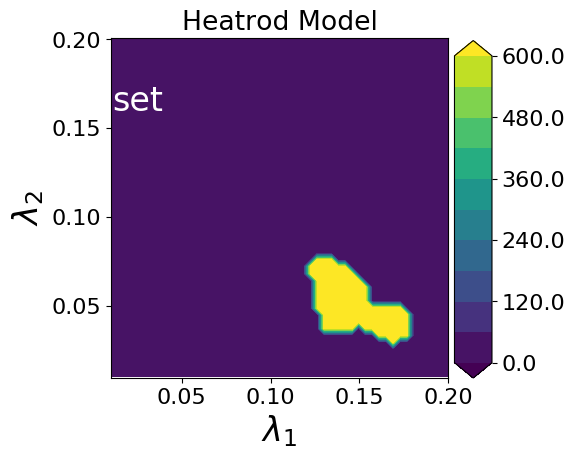
\includegraphics[width=\linewidth]{examples/fig_heatrod_q1/HeatrodModel--set_N50_em.png}
\end{minipage}
\begin{minipage}{.475\textwidth}
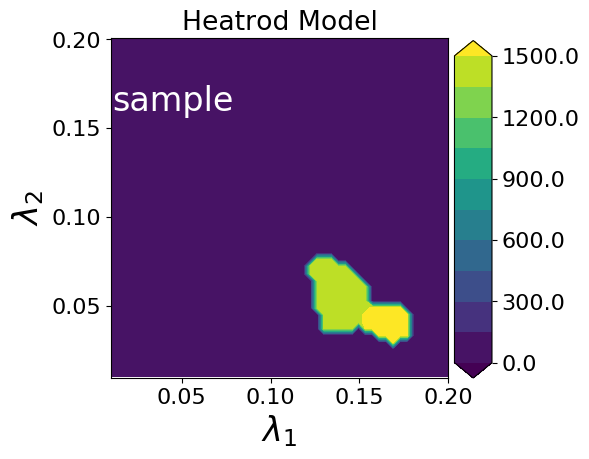
\includegraphics[width=\linewidth]{examples/fig_heatrod_q1/HeatrodModel--sample_N50_mc.png}
\end{minipage}
\caption{The inverse image of the reference measure for set-based (left) and sample-based (right) solutions for $N=50$ parameter samples.}
\label{fig:heatrod-sol-ex}
\end{figure}



